%%%%%%%%%%%%%%%%%%%%%%%%%%%%%%%%%%%%%%%%%%%%%%%%%%%%%%%%%%%%%%%%%%%%%%%%
% Uni Duesseldorf
% Lehrstuhl fuer Datenbanken und Informationssysteme
% Vorlage fuer Bachelor-/Masterarbeiten
% Optimiert fuer den Original-Latex-Kompiler LATEX.EXE (LaTeX=>PS=>PDF)
%%%%%%%%%%%%%%%%%%%%%%%%%%%%%%%%%%%%%%%%%%%%%%%%%%%%%%%%%%%%%%%%%%%%%%%%
% Ueberarbeitung für pdflatex (LaTeX=>PDF)
%%%%%%%%%%%%%%%%%%%%%%%%%%%%%%%%%%%%%%%%%%%%%%%%%%%%%%%%%%%%%%%%%%%%%%%%
% Vorlage Changelog:
% 10.09.2015 (Matthias Liebeck): Nummerierung des Inhaltsverzeichnis nun römisch, Beispiel für einen Anhang eingebaut, \raggedbottom hinter sections eingefügt
%%%%%%%%%%%%%%%%%%%%%%%%%%%%%%%%%%%%%%%%%%%%%%%%%%%%%%%%%%%%%%%%%%%%%%%%
%%%% BEGINN EINSTELLUNG FUER DIE ARBEIT. UNBEDINGT ERFORDERLICH! %%%%%%%
%%%%%%%%%%%%%%%%%%%%%%%%%%%%%%%%%%%%%%%%%%%%%%%%%%%%%%%%%%%%%%%%%%%%%%%%
% Geben Sie Ihren Namen hier an:
\newcommand{\bearbeiter}{Fabian Ruhland}

% Geben Sie hier den Titel Ihrer Arbeit an:
\newcommand{\titel}{Eine Toolbox zur Simulation und Visualisierung von Automaten und Grammatiken}

% Geben Sie das Datum des Beginns und Ende der Bachelorarbeit ein:
\newcommand{\beginndatum}{27. Juni 2016}
\newcommand{\abgabedatum}{27.~September~2016}

% Geben Sie die Namen des Erst- und Zweitgutachters an:
\newcommand{\erstgutachter}{Prof. Dr.~Michael Leuschel}
\newcommand{\zweitgutachter}{Prof. Dr.~J\"org Rothe}

% Falls Sie die Arbeit zweiseitig ausdrucken wollen,
% benutzen Sie die folgende Zeile mit
% \AN fuer zweiseitigen Druck
% \AUS fuer einseitigen Druck
\newcommand{\zweiseitig}{\AN}

% Falls die Arbeit in englischer Sprache verfasst 
% werden soll, dann benutzen Sie die folgende Zeile mit
% englisch fuer englische Sprache
% deutsch fuer deutsche Sprache
\newcommand{\sprache}{deutsch}

% Hier wird eingestellt, ob es sich bei der Arbeit um eine Bachelor- 
% oder Masterarbeit handelt (unpassendes auskommentieren!):
\newcommand{\arbeit}{Bachelorarbeit}
%~ \newcommand{\arbeit}{Masterarbeit}


%%%%%%%%%%%%%%%%%%%%%%%%%%%%%%%%%%%%%%%%%%%%%%%%%%%%%%%%%%%%%%%%%%%%%%%%
%%%% ENDE EINSTELLUNGEN %%%%%%%%%%%%%%%%%%%%%%%%%%%%%%%%%%%%%%%%%%%%%%%%
%%%%%%%%%%%%%%%%%%%%%%%%%%%%%%%%%%%%%%%%%%%%%%%%%%%%%%%%%%%%%%%%%%%%%%%%

% Die folgende Zeile NICHT EDITIEREN oder loeschen


%%%%%%%%%%%%%%%%%%%%%%%%%%%%%%%%%%%%%%%%%%%%%%%%%%%%%%%%%%%
% Obere Titelmakros. Editieren Sie diese Datei nur, wenn
% Sie sich ABSOLUT sicher sind, was Sie da tun!!!
% (Z.B. zum Abaendern der BA-Vorlage in eine MA-Vorlage)
% Uni Duesseldorf
% Lehrstuhl fuer Datenbanken und Informationssysteme
% Version 2.2 - 2.3.2010
%%%%%%%%%%%%%%%%%%%%%%%%%%%%%%%%%%%%%%%%%%%%%%%%%%%%%%%%%%%
\newcommand{\AN}{twoside}
\newcommand{\AUS}{}
%\newcommand{\englisch}{}
%\newcommand{\deutsch}{\usepackage[german]{babel}}

%% Die folgenden auskommentierten Optionen dienen der automatischen
%% Erkennung des Latex-Kompilers und dem Setzen der davon abhängigen
%% Einstellungen. Bei Problem z.B. mit dem Einbinden von verschiedenen
%% Grafiktypen bei Verwendung von PdfLatex oder Latex, einfach die
%% verschiedenen \usepackage(s) ausprobieren. (Mit diesen Einstellungen
%% funktionierte diese Vorlage bei der Verwenundg von latex.exe als
%% Kompiler bei den meisten Studierenden.)

%\newif\ifpdf \ifx\pdfoutput\undefined
%\pdffalse % we are not running pdflatex
%\else
%\pdfoutput=1 % we are running pdflatex
%\pdfcompresslevel=9 % compression level for text and image;
%\pdftrue \fi

\documentclass[11pt,a4paper, \zweiseitig]{article}



%\usepackage[iso]{umlaute}
\usepackage[utf8, ansinew]{inputenc}
\usepackage{palatino} % palatino Schriftart
%\usepackage{makeidx} % um ein Index zu erstellen
\usepackage[T1]{fontenc} %fuer richtige Trennung bei Umlauten
\usepackage{fancybox} % fuer die Rahmen
\usepackage{shortvrb}
\usepackage{ifthen}
\usepackage{color}
\usepackage{amssymb}
\usepackage{amsmath,amsthm}
\usepackage{listings}
\usepackage{color}
\ifthenelse{\equal{\sprache}{deutsch}}{\usepackage[ngerman]{babel}}{}
\usepackage{a4wide} % ganze A4 Weite verwenden
\usepackage{verbatim}
%\usepackage{algorithm2e}
\usepackage{algorithm,algorithmic}
\usepackage{float}
%\ifpdf
%\usepackage[pdftex,xdvi]{graphicx}
%\usepackage{thumbpdf} %thumbs fuer Pdf
%\usepackage[pdfstartview=FitV]{hyperref} %anklickbares Inhaltsverzeichnis
%\else
%\usepackage[dvips,xdvi]{graphicx}
\usepackage{graphicx}
\usepackage{hyperref} %anklickbares Inhaltsverzeichnis
%\fi
\usepackage{tikz}
\usetikzlibrary{automata,positioning}

%%%%%%%%%%%%%%%%%%%%%%% Massangaben fuer die Arbeit %%%%%%%%%%%%%%%
\setlength{\textwidth}{15cm}

\setlength{\oddsidemargin}{35mm}
\setlength{\evensidemargin}{25mm}

\addtolength{\oddsidemargin}{-1in}
\addtolength{\evensidemargin}{-1in}

%\makeindex

\begin{document}

\renewcommand{\algorithmicrequire}{\textbf{Input:}}
\renewcommand{\algorithmicensure}{\textbf{Output:}}
\renewcommand{\listalgorithmname}{Algorithmenverzeichnis}
%\setcounter{secnumdepth}{4} %Nummerieren bis in die 4. Ebene
%\setcounter{tocdepth}{4} %Inhaltsverzeichnis bis zur 4. Ebene

\pagestyle{headings}

\sloppy % LaTeX ist dann nicht so streng mit der Silbentrennung
%~ \MakeShortVerb{\§}

\parindent0mm
\parskip0.5em


{
\textwidth170mm 
\oddsidemargin30mm 
\evensidemargin30mm 
\addtolength{\oddsidemargin}{-1in}
\addtolength{\evensidemargin}{-1in}

\parskip0pt plus2pt

% Die Raender muessen eventuell fuer jeden Drucker individuell eingestellt
% werden. Dazu sind die Werte fuer die Abstaende `\oben' und `\links' zu
% aendern, die von mir auf jeweils 0mm eingestellt wurden.

%\newlength{\links} \setlength{\links}{10mm}  % hier abzuaendern
%\addtolength{\oddsidemargin}{\links}
%\addtolength{\evensidemargin}{\links}

\begin{titlepage}
\vspace*{-1.5cm}
  \raisebox{17mm}{
    \begin{minipage}[t]{70mm}
      \begin{center}
        %\selectlanguage{german}
        {\Large INSTITUT F�R INFORMATIK\\}
        {\normalsize
          Datenbanken und Informationssysteme\\
        }
        \vspace{3mm}
        {\small Universit�tsstr. 1 \hspace{5ex} D--40225 D�sseldorf\\}
     \end{center}
    \end{minipage}
  }
  \hfill
  
\includegraphics[width=130pt]{bilder/HHU_Logo}
  \vspace{14em}

% Titel
  \begin{center}
      	\baselineskip=55pt
    	\textbf{\huge \titel}
  	 	\baselineskip=0 pt
   \end{center}

  %\vspace{7em}

\vfill

% Autor
  \begin{center}
    \textbf{\Large
      \bearbeiter
    }
  \end{center}

  \vspace{35mm}
 
% Prüfungsordnungs-Angaben
  \begin{center}
    %\selectlanguage{german}
    
%%%%%%%%%%%%%%%%%%%%%%%%%%%%%%%%%%%%%%%%%%%%%%%%%%%%%%%%%%%%%%%%%%%%%%%%%
% Ja, richtig, hier kann die BA-Vorlage zur MA-Vorlage gemacht werden...
% (nicht mehr nötig!)
%%%%%%%%%%%%%%%%%%%%%%%%%%%%%%%%%%%%%%%%%%%%%%%%%%%%%%%%%%%%%%%%%%%%%%%%%
    {\Large \arbeit}

    \vspace{2em}

    \begin{tabular}[t]{ll}
      Beginn der Arbeit:& \beginndatum \\
      Abgabe der Arbeit:& \abgabedatum \\
      Gutachter:         & \erstgutachter \\
                         & \zweitgutachter \\
    \end{tabular}
  \end{center}

\end{titlepage}

}

%%%%%%%%%%%%%%%%%%%%%%%%%%%%%%%%%%%%%%%%%%%%%%%%%%%%%%%%%%%%%%%%%%%%%
\clearpage
\begin{titlepage}
  ~                % eine leere Seite hinter dem Deckblatt
\end{titlepage}
%%%%%%%%%%%%%%%%%%%%%%%%%%%%%%%%%%%%%%%%%%%%%%%%%%%%%%%%%%%%%%%%%%%%%
\clearpage
\begin{titlepage}
\vspace*{\fill}

\section*{Erkl�rung}

%%%%%%%%%%%%%%%%%%%%%%%%%%%%%%%%%%%%%%%%%%%%%%%%%%%%%%%%%%%
% Und hier ebenfalls ggf. BA durch MA ersetzen...
% (Auch nicht mehr nötig!)
%%%%%%%%%%%%%%%%%%%%%%%%%%%%%%%%%%%%%%%%%%%%%%%%%%%%%%%%%%%

Hiermit versichere ich, dass ich diese \arbeit~
selbstst�ndig verfasst habe. Ich habe dazu keine anderen als die
angegebenen Quellen und Hilfsmittel verwendet.

\vspace{25 mm}

\begin{tabular}{lc}
D�sseldorf, den \abgabedatum \hspace*{2cm} & \underline{\hspace{6cm}}\\
& \bearbeiter
\end{tabular}

\vspace*{\fill}
\end{titlepage}

%%%%%%%%%%%%%%%%%%%%%%%%%%%%%%%%%%%%%%%%%%%%%%%%%%%%%%%%%%%%%%%%%%%%%
% Leerseite bei zweiseitigem Druck
%%%%%%%%%%%%%%%%%%%%%%%%%%%%%%%%%%%%%%%%%%%%%%%%%%%%%%%%%%%%%%%%%%%%%

\ifthenelse{\equal{\zweiseitig}{twoside}}{\clearpage\begin{titlepage}
~\end{titlepage}}{}

%%%%%%%%%%%%%%%%%%%%%%%%%%%%%%%%%%%%%%%%%%%%%%%%%%%%%%%%%%%%%%%%%%%%%
\clearpage
\begin{titlepage}

%%% Die folgende Zeile nicht ändern!
\section*{\ifthenelse{\equal{\sprache}{deutsch}}{Zusammenfassung}{Abstract}}
%%% Zusammenfassung:
Hier kommt eine ca.\ einseitige Zusammenfassung der Arbeit rein.



%%%%%%%%%%%%%%%%%%%%%%%%%%%%%%%%%%%%%%%%%%%%%%%%
% Untere Titelmakros. Editieren Sie diese Datei nur, wenn Sie sich
% ABSOLUT sicher sind, was Sie da tun!!!
%%%%%%%%%%%%%%%%%%%%%%%%%%%%%%%%%%%%%%%%%%%%%%%
\vspace*{\fill}
\end{titlepage}

%%%%%%%%%%%%%%%%%%%%%%%%%%%%%%%%%%%%%%%%%%%%%%%%%%%%%%%%%%%%%%%%%%%%%
% Leerseite bei zweiseitigem Druck
%%%%%%%%%%%%%%%%%%%%%%%%%%%%%%%%%%%%%%%%%%%%%%%%%%%%%%%%%%%%%%%%%%%%%
\ifthenelse{\equal{\zweiseitig}{twoside}}
  {\clearpage\begin{titlepage}~\end{titlepage}}{}
%%%%%%%%%%%%%%%%%%%%%%%%%%%%%%%%%%%%%%%%%%%%%%%%%%%%%%%%%%%%%%%%%%%%%
\clearpage \setcounter{page}{1}
\pagenumbering{roman}
\setcounter{tocdepth}{3}
\tableofcontents

%\enlargethispage{\baselineskip}
\clearpage
%%%%%%%%%%%%%%%%%%%%%%%%%%%%%%%%%%%%%%%%%%%%%%%%%%%%%%%%%%%%%%%%%%%%%
% Leere Seite, falls Inhaltsverzeichnis mit ungerader Seitenzahl und 
% doppelseitiger Druck
%%%%%%%%%%%%%%%%%%%%%%%%%%%%%%%%%%%%%%%%%%%%%%%%%%%%%%%%%%%%%%%%%%%%%
\ifthenelse{ \( \equal{\zweiseitig}{twoside} \and \not \isodd{\value{page}} \)}
	{\pagebreak \thispagestyle{empty} \cleardoublepage}{\clearpage}



\pagenumbering{arabic}
\setcounter{page}{1}

%%%%%%%%%%%%%%%%%%%%%%%%%%%%%%%%%%%%%%%%%%%%%%%%%%%%%%%%%%%%%%%%%%%%%%%%
%%%% BEGINN TEXTTEIL %%%%%%%%%%%%%%%%%%%%%%%%%%%%%%%%%%%%%%%%%%%%%%%%%%%
%%%%%%%%%%%%%%%%%%%%%%%%%%%%%%%%%%%%%%%%%%%%%%%%%%%%%%%%%%%%%%%%%%%%%%%%

%%%%%%%%%%%%%%%%%%%%%%%%%%%%%%%%%%%%%%%%%%%%%%%%%%%%%%%%%%%%%%%%%%%%%%%%
% Text entweder direkt hier hinein schreiben oder, im Sinne der
% besseren Uebersichtlich- und Bearbeitbarkeit mittels \input die
% einzelnen Textteile hier einbinden.
%%%%%%%%%%%%%%%%%%%%%%%%%%%%%%%%%%%%%%%%%%%%%%%%%%%%%%%%%%%%%%%%%%%%%%%%

\section{Einleitung}\raggedbottom
\label{sec:1}
Im Folgenden Abschnitt werden zunächst einmal Grammatiken und Automaten definiert und anhand eines kurzen Beispiels erläutert. Die hier verwendeten Definitionen sind an das Drachenbuch\cite{DraBu} angelehnt.
\subsection{Grammatiken}
\label{sec:1.1}
Eine Grammatik setzt sich aus den vier folgenden Bestandteilen zusammen:
\begin{itemize}
	\item Einer Menge von Terminalen. Terminale sind die Symbole, welche die von der Grammatik erzeugten Sprache ausmachen.
	\item Einer Menge von Nichtterminalen. Jedes Nichtterminal wird mit einer Produktion auf eine Liste von weiteren Terminalen und Nichtterminalen abgebildet, so dass durch wiederholte Anwendung dieser Produktionen Terminalstrings (Wörter) entstehen.
	\item Einer Menge von Produktionen. Eine Produktion hat drei Bestandteile: Ein Nichtterminal auf der linken Seite, einen Pfeil in der Mitte und eine Reihe von Terminalen und Nichtterminalen auf der rechten Seite. Die Produktionen beschreiben wie die Terminale und Nichtterminale zu Wörtern zusammengesetzt werden, die nur noch Terminale enthalten.
	\item Einem Startsymbol. Eines der Nichtterminale wird als Startsymbol ausgewiesen. Bei der Bildung eines Wortes wird immer mit einer der Regeln des Startsymbols begonnen.
\end{itemize}
Ein Beispiel für eine Grammatik wäre:
\lstset{
	captionpos=b,
	breaklines=true,
}
\begin{lstlisting}[frame=single, caption=Beispiel für eine Grammatik]
{a, b; S, A; S}

S --> aA
A --> aA
A --> b
\end{lstlisting}
Diese Grammatik besteht aus den Terminalen a und b, den Nichtterminalen S und A, wobei S das Startsymbol der Grammatik ist, und den drei aufgelisteten Produktionen. Die von dieser Grammatik erzeugten Wörter sind sehr einfach:\\
Man beginnt mit dem Startsymbol S und leitet es nach aA ab. Anschließend kann man das A beliebig oft nach aA ableiten und um das Wort abzuschließen leitet man es einmal nach b ab. Es entstehen also Wörter wie zum Beispiel \textit{ab}, \textit{aab}, \textit{aaaaaab}, etc.
\subsection{Automaten}
\label{sec:1.2}
Bei Automaten unterscheiden wir zwischen deterministischen und nichtdeterministischen endlichen Automaten. Diese beiden Formen von Automaten sind sich sehr ähnlich: Deterministische Automaten weisen jedoch eine bedeutende Einschränkung im Vergleich zu nichtdeterministischen Automaten auf. Beide sind Akzeptoren, das heißt sie können ein Eingabewort entweder akzeptieren oder nicht.
\\
Ein nichtdeterministischer endlicher Automat (NFA) besteht aus:
\begin{itemize}
	\item Einer endlichen Menge von Zuständen
	\item Einer Menge von Eingabesymbolen (dem Eingabealphabet). Diese entsprechen den Terminalsymbolen bei einer Grammatik.
	\item Einer Übergangsfunktion, die für jeden Zustand und jedes Symbol aus dem Eingabealphabet eine Menge von nächsten Zuständen ausgibt.
	\item Einem Startzustand. Hierzu wird ein Zustand des Automaten als Startzustand ausgewiesen.
	\item Einer Menge von Endzuständen. Wenn die Übergangsfunktion für ein bestimmtes Eingabewort einen dieser Zustände ausgibt, wird das Wort vom Automaten akzeptiert.
\end{itemize}
Ein deterministischer endlicher Automat (DFA) besteht aus den gleichen Komponenten. Jedoch muss die Übergangsfunktion hier für einen Zustand und ein Eingabesymbol aus dem Eingabealphabet nur genau einen nächsten Zustand ausgeben, im Gegensatz zu einem NFA, bei dem sie eine Menge von Zuständen ausgibt, die auch leer sein kann.\\
NFAs und DFAs können durch einen gerichteten Graph dargestellt werden. Die Knoten dieses Graphen sind die Zustände des jeweiligen Automaten und die Kanten stehen für seine Übergangsfunktion. Man nennt diesen Graph \textit{Übergangsgraph}.\\
Der folgende Automat mit dem Eingabealphabet \{a, b\} und der Zustandsmenge \{z0, z1, z2\} akzeptiert die von der oben gezeigten Grammatik erzeugte Sprache.
\begin{figure}[H]
	\centering
	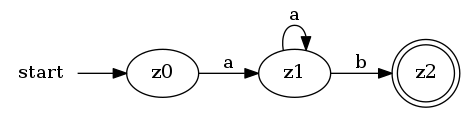
\includegraphics[width=0.75\textwidth]{bilder/beispiel_automat1.png}
	\caption{Beispiel für einen DFA}
	\label{fig:pic1}
\end{figure}
Wie man erkennt, wird z0 durch einen Startpfeil als Startzustand und z2 durch einen doppelten Kreis als Endzustand markiert.
\newpage
\section{Bedienung des Programms}\raggedbottom
\label{sec:2}
Im folgenden Abschnitt soll die Bedienung der Toolbox genauer erläutert werden. Hierzu werden zunächst die Eingabeformate für die Grammatiken und Automaten beschrieben. Anschließend folgt ein Überblick über die Bedienung des Programms in der Konsole und zum Schluss wird die Bedienung der graphischen Oberfläche erläutert.
\subsection{Eingabeformat für Grammatiken}
\label{sec:2.1}
Grammatiken werden in ganz normalen Textdateien gespeichert.\\
Zu Beginn einer solchen Textdatei stehen immer die Terminal- und Nichtterminalmengen, sowie das Startsymbol. Das sieht wie folgt aus:
\lstset{
	captionpos=b,
	breaklines=true,
}
\begin{lstlisting}[frame=single, caption=Definition der Termiale und Nichtterminale]
{'a', 'b', 'c'; S, A, B; S}
\end{lstlisting}
Wie man sieht, werden die Terminale in einfache Anführungszeichen geschrieben. Ein Terminal kann eine beliebig lange Zeichenkette sein, die alle Unicode-Charaktere außer dem einzelnen Hochkomma enthalten darf. Ein Nichtterminal ist ebenfalls eine beliebig lange Zeichenkette, jedoch darf diese nur Kleinbuchstaben, Großbuchstaben, Zahlen und den Unterstrich enthalten, und darf nicht mit einer Zahl beginnen. Nach der Menge von Terminalen und der Menge von Nichtterminalen folgt jeweils ein Semikolon.\\
Anschließend folgen die Produktionen, welche so aussehen:
\begin{lstlisting}[frame=single, caption=Beispiel für eine Produktion in einer Grammatik]
A --> 'A', 'a'
\end{lstlisting}
Links steht ein Nichtterminal, dann folgt ein Pfeil und anschließend eine Liste von Terminalen und Nichtterminalen, die jeweils durch Kommata separiert sind. Hierbei ist es wichtig, dass sowohl die Terminale, als auch die Nichtterminale in einfachen Hochkommata stehen.\\
Eine vollständige Grammatik könnte zum Beispiel so aussehen:
\begin{lstlisting}[frame=single, caption=Beispiel für eine Grammatik]
{'a', 'b', 'c'; S, A, B; S}

S --> 'A', 'B'
A --> 'A', 'a'
A --> 'a'
B --> 'B', 'b'
B --> 'b'
\end{lstlisting}
\subsection{Eingabeformat von Automaten}
\label{sec:2.2}
Automaten werden ebenfalls in einfachen Textdateien gespeichert. Das Eingabeformat ist sehr ähnlich zu dem der Grammatiken.\\
Zunächst werden die Zustandsmenge, anschließend der Startzustand und zum Schluss die Endzustände des Automaten deklariert:
\begin{lstlisting}[frame=single, caption=Definition der Zustände]
{z0, z1, z2; z0; z2}
\end{lstlisting}
Der Name eines Zustandes kann beliebig lang sein und darf Kleinbuchstaben, Großbuchstaben, Zahlen und den Unterstrich enthalten, jedoch nicht mit einer Zahl anfangen. Nach der Menge der Zustände und dem Startzustand folgt jeweils ein Semikolon.\\
Nun folgen die Regeln der Übergangsfunktion:
\begin{lstlisting}[frame=single, caption=Beispiel für eine Produktion eines Automaten]
z0 --'a','b'--> z1
\end{lstlisting}
Links steht der Name des Zustands, von dem die Regel ausgeht. Es folgt ein Pfeil, in dessen Mitte die Menge an Eingabesymbolen steht, für die die Übergangsfunktion in den nächsten Zustand geht. Dieser befindet sich rechts des Pfeils befindet. Die Eingabesymbole können beliebig lang sein und sich aus allen Unicode-Charakteren, außer dem einzelnen Hochkomma, zusammensetzen und müssen selbst zwischen zwei einzelnen Hochkommata stehen.\\
Hier ist ein Beispiel für einen vollständigen Automaten:
\begin{lstlisting}[frame=single, caption=Beispiel für einen Automaten]
{z0, z1, z2; z0; z2}

z0 --'a'--> z1
z1 --'a'--> z1
z1 --'b'--> z2
z2 --'b'--> z2
\end{lstlisting}
Der daraus resultierende Automat sieht so aus:
\begin{figure}[H]
	\centering
	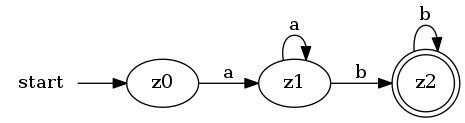
\includegraphics[width=0.75\textwidth]{bilder/beispiel_automat2.png}
	\caption{Beispiel für einen Automaten}
	\label{fig:pic2}
\end{figure}
\newpage
\subsection{Bedienung des Programms in der Konsole}
\label{sec:2.3}
Nach dem Start des Programms in einem Terminal wird man so begrüßt:
\begin{figure}[H]
	\centering
	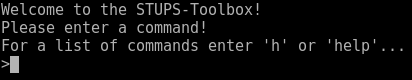
\includegraphics[width=0.75\textwidth]{bilder/konsole1.png}
	\caption{So sieht das Programm direkt nach dem Start aus}
	\label{fig:pic3}
\end{figure}
Nun hat man die Möglichkeit eine Reihe von Befehlen einzutippen, welche im folgenden aufgelistet und kurz erklärt werden.
\begin{itemize}
	\item Befehle des Hauptprogramms:
	\begin{itemize}
		\item \textit{help} oder \textit{h}:\\
		Listet alle verfügbaren Befehle mit einer kurzen Beschreibung ihrer jeweiligen Funktion auf.
		\item \textit{gui}:\\
		Öffnet die grafische Oberfläche des Programms. Die Konsole wird eingefroren, solange die grafische Oberfläche geöffnet ist und kann wieder benutzt werden, wenn sie geschlossen wird.
		\item \textit{about} oder \textit{a}:\\
		Zeigt Informationen über den aktuellen Release des Programms an.
		\item \textit{exit} oder \textit{e}:
		Beendet das Programm.
	\end{itemize}
\end{itemize}
\begin{itemize}
	\item Befehle für Grammatiken:
	\begin{itemize}
		\item \textit{load-grammar} oder \textit{lg}:\\
		Nimmt als einzigen Parameter einen Dateinamen, oder den Pfad zu einer Datei. Diese Datei sollte eine Grammatik in der in Abschnitt \hyperref[sec:2.1]{2.1} beschriebenen Form enthalten und wird dann vom Programm eingelesen und geladen.
		\item \textit{save-grammar} oder \textit{sg}:\\
		Nimmt als einzigen Parameter einen Dateinamen, oder den Pfad zu einer Datei. Die aktuell geladene Grammatik wird in dieser Datei in dem in Abschnitt \hyperref[sec:2.1]{2.1} beschriebenen Format gespeichert.
		\item \textit{print-grammar} oder \textit{pg}:\\
		Gibt die aktuell geladene Grammatik auf der Konsole aus.
		\item \textit{nullable}:\\
		Berechnet die nullable-Menge (die Menge aller Nichtterminale, die auf das leere Wort abgebildet werden können) der aktuell geladenen Grammatik und gibt sie auf der Konsole aus.
		\item \textit{first}:\\
		Berechnet die First-Menge jedes Nichtterminals der aktuell geladenen Grammatik und gibt sie auf der Konsole aus.
		\item \textit{follow}:\\
		Berechnet die Follow-Menge jedes Nichtterminals der aktuell geladenen Grammatik und gibt sie auf der Konsole aus.
	\end{itemize}
\end{itemize}
\begin{itemize}
	\item Befehle für Automaten:
	\begin{itemize}
		\item \textit{load-automaton} oder \textit{la}:\\
		Nimmt als einzigen Parameter einen Dateinamen, oder den Pfad zu einer Datei. Diese Datei sollte einen Automaten in der in Abschnitt \hyperref[sec:2.2]{2.2} beschriebenen Form enthalten und wird dann vom Programm eingelesen und geladen.
		\item \textit{save-grammar} oder \textit{sg}:\\
		Nimmt als einzigen Parameter einen Dateinamen, oder den Pfad zu einer Datei. Der aktuell geladene Automat wird in dieser Datei in dem in Abschnitt \hyperref[sec:2.2]{2.2} beschriebenen Format gespeichert.
		\item \textit{print-automaton} oder \textit{pa}:\\
		Gibt den aktuell geladenen Automaten auf der Konsole aus.
		\item \textit{graph-automaton} oder \textit{ga}:\\
		Nimmt als einzigen Parameter einen Dateinamen, oder den Pfad zu einer Datei. Der aktuell geladene Automat wird in dieser Datei im GraphViz-Format gespeichert.
		\item \textit{check-string-automaton} oder \textit{csa}:\\
		Nimmt als einzigen Parameter einen Eingabestring und prüft, ob dieser von dem aktuell geladenen Automaten akzeptiert wird. Der Eingabestring muss zwischen zwei Anführungszeichen stehen und die Eingabesymbole durch Leerzeichen getrennt sein (zum Beispiel: \textit{csa "'a a a b b c"'}).
		\item \textit{rename-states} oder \textit{rs}:\\
		Benennt die Zustände des aktuell geladenen Automaten um, so dass diese nur kurze, übersichtliche Namen haben.
		\item \textit{remove-epsilon-transitions}, oder \textit{ret}:\\
		Wandelt den aktuell geladenen Automaten in einen Automaten ohne Epsilon-Übergänge um.
		\item \textit{convert-to-dfa} oder \textit{todfa}:\\
		Wandelt den aktuell geladenen Automaten in einen DFA um. \textit{Achtung}: Der hieraus resultierende Automat hat keine vollständige Übergangsfunktion und ist somit streng genommen kein richtiger DFA. Da viele Automaten jedoch sehr unübersichtlich werden, nachdem ihre Übergangsfunktion vervollständigt wurde, habe ich mich dazu entschlossen, hierfür einen zusätzlichen Befehl hinzuzufügen.
		\item \textit{complete-automaton} oder \textit{ca}:\\
		Wandelt den aktuell geladenen Automaten in einen DFA mit einer vollständigen Übergangsfuntkion um.
		\item \textit{minimize-dfa} oder \textit{min}:\\
		Wandelt den aktuell geladenen Automaten in einen minimierten DFA um. Vor dem Umwandeln werden die Zustände des Automaten automatisch neu benannt, damit es beim Verschmelzen der Zustände nicht zu unübersichtlich wird.
	\end{itemize}
\end{itemize}
\subsection{Bedienung der grafischen Oberfläche}
\label{sec:2.4}
Durch eintippen des Befehls \textit{gui} öffnet sich ein Fenster. Hier hat man nun die Möglichkeit im \textit{Choose Plugin}-Menü eine grafische Oberfläche für Grammatiken oder Automaten auszuwählen.
\subsubsection{Grammatiken}
\label{sec:2.4.1}
Die Grammatik-Main.GUI startet in der Bearbeitungsoberfläche. Hier wird die aktuell geladene Grammatik angezeigt und kann bearbeitet werden.
\begin{figure}[H]
	\centering
	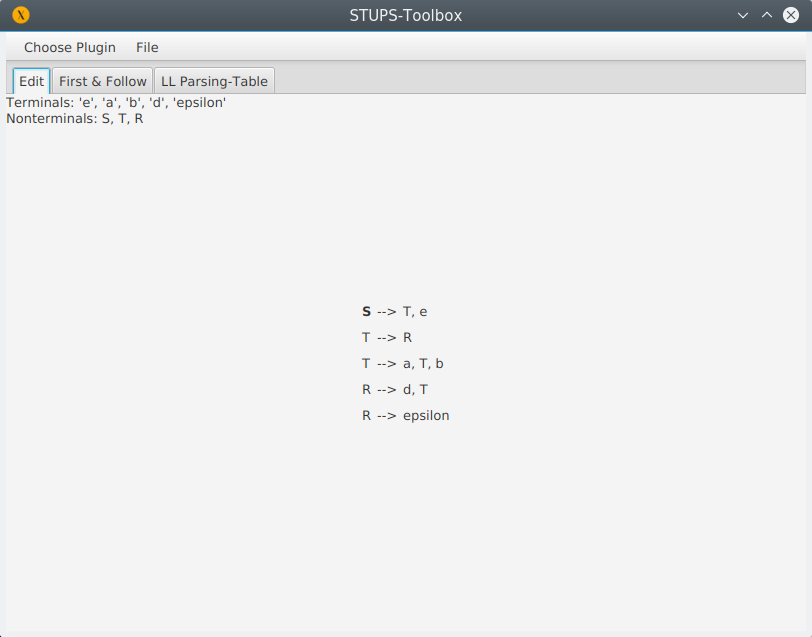
\includegraphics[width=0.75\textwidth]{bilder/gui1.png}
	\caption{Die grafische Oberfläche zeigt eine Grammatik an}
	\label{fig:pic4}
\end{figure}
\paragraph{Bedienung der Oberfläche}\ \\
Zusätzlich zum \textit{Choose Plugin}-Menü befindet sich nun noch das \textit{File}-Menü, mit welchem es möglich ist, eine neue Grammatik zu erstellen, eine Grammatik zu öffnen und die aktuelle Grammatik zu speichern.
Unter der Menüleiste sind einige Reiter zu sehen:\\
\begin{itemize}
	\item Edit:\\
	Hier wird die aktuelle Grammatik angezeigt und kann bearbeitet werden. Das Startsymbol ist fettgedruckt.
	\item First \& Follow:\\
	Hier werden nullable-, First- und Follow-Mengen der Grammatik angezeigt.
	\item LL Parsing-Table:\\
	Diese Oberfläche zeigt die LL Parser-Tabelle für die aktuelle Grammatik an. Konflikte werden rot markiert.
\end{itemize}
\paragraph{Bearbeiten einer Grammatik}\ \\
Durch Rechtsklick auf ein Nichtterminal öffnet sich ein Kontextmenü mit den Optionen \textit{Edit Symbol}, \textit{Delete Symbol} und \textit{Set as Start Symbol}.\\
Durch Auswahl von \textit{Edit Symbol} erscheint ein Textfeld anstelle des Nichtterminals, in welches man einen neuen Namen für dieses eingeben kann. Dieser Effekt wird auch durch einen Doppelklick auf das Nichtterminal erreicht.\\
Mit Klick auf \textit{Delete Symbol} wird das Nichtterminal aus der Grammatik entfernt. Dadurch werden auch alle Produktionen, bei denen es auf der linken Seite steht, entfernt.\\
\textit{Set as Start Symbol} hat zur Folge, dass das ausgewählte Nichtterminal nun das Startsymbol der Grammatik ist.\\
Auch durch Rechtsklick auf die Liste von Terminalen und Nichtterminalen öffnet sich ein Kontextmenü. Dieses hat die Einträge \textit{Edit List} und \textit{Delete Rule}.\\
\textit{Edit List} hat einen ähnlichen Effekt wie \textit{Edit Symbol}, nur dass man hier die Symbolliste bearbeiten kann. Die Symbole müssen bei der Eingabe durch Kommata getrennt sein. Auch hier ist es möglich, einfach doppelt auf die Liste zu klicken, um sie zu bearbeiten.\\
Mit \textit{Delete Rule} wird die ausgewählte Produktion aus der Grammatik entfernt. Falls in der Liste Symbole vorkommen, die in sonst keiner Produktion sind, werden diese auch aus der Grammatik entfernt.\\
Per Rechtsklick in die leere Fläche öffnet man ein Kontextmenü, dass nur den Eintrag \textit{Add Rule} enthält. Dieser öffnet ein Fenster, in welchem man eine neue Produktion erstellen kann. Hierzu müssen die linke und die rechte Seite dieser Produktion angegeben werden.
\newpage
\subsubsection{Automaten}
\label{sec:2.4.2}
Im Gegensatz zu der Grammatikoberfläche, hat die Main.GUI für Automaten nur eine einzige Oberfläche auf der alle Funktionen vereint sind.
\begin{figure}[H]
	\centering
	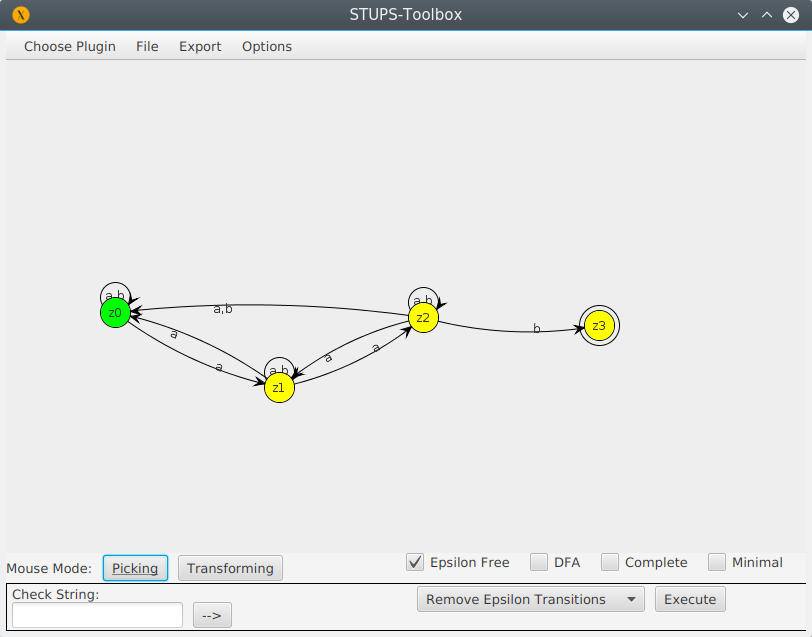
\includegraphics[width=0.75\textwidth]{bilder/gui2.png}
	\caption{Die grafische Oberfläche zeigt einen Automaten an}
	\label{fig:pic5}
\end{figure}
Auch hier finden sich neue Menüeinträge neben \textit{Choose Plugin}. Diese sind \textit{File}, womit man einen neuen Automaten erstellen, einen Automaten aus einer Datei öffnen und eine Automaten in eine Datei speichern kann, \textit{Export}, welcher es ermöglicht einen Automaten im GraphViz-Format zu speichern, und \textit{Options}, welcher zwei weitere Menüs beinhaltet, mit denen man das Layout des Übergangsgraphen und die Farben der Zustände und Produktionen anpassen kann.\\
\paragraph{Bearbeiten eines Automaten}\ \\
Im Zentrum des Fensters wird der geladene Automat angezeigt. Durch Rechtsklick auf einen Zustand, einen Produktionspfeil oder in die leere Fläche, öffnet sich ein Kontextmenü, welches, je nachdem wohin geklickt wurde, unterschiedliche Menüpunkte zum Bearbeiten des Automaten anbietet. So ist es möglich neue Zustände und Produktionen hinzuzufügen, bzw. bereits vorhandene Zustände und Produktionen zu verändern.\\
Unterhalb des Automaten sind zwei Knöpfe, mit denen man die Funktion der Maus festlegen kann. Standardmäßig ist \textit{Picking} aktiviert. In diesem Modus kann man einzelne Zustände mit der linken Maustaste auswählen und verschieben. Man kann auch mehrere Zustände auf einmal auswählen und verschieben, in dem man die linke Maustaste gedrückt hält und den Mauszeiger über die gewünschten Zustände zieht.\\
Der zweite Modus \textit{Transforming} erlaubt es den ganzen Automaten zu verschieben und zu transformieren. In dem man die linke Maustaste gedrückt hält und den Mauszeiger bewegt, kann man den Übergangsgraphen verschieben. Hält man zusätzlich noch die Strg-Taste gedrückt, kann der Graph gestreckt, bzw. gestaucht werden. Mit der Umschalt-Taste ist es möglich den Graphen zu drehen.\\
In beiden Modi lässt sich das Scrollrad der Maus benutzen um rein- und raus zu zoomen.\\
Rechts neben den beiden Knöpfen gibt es noch vier Indikatoren, die angeben, ob der angezeigte Automat frei von Epsilon-Übergängen ist, ob er ein DFA ist, ob seiner Übergangsfunktion vollständig ist, und ob er ein DFA mit einer minimalen Übergangsfunktion ist.
Im unteren Bereich des Fensters werden die geladenen Funktions-Plugins angezeigt. Hierbei wird zwischen Plugins mit eigener grafischen Oberfläche und solchen, die einfach nur eine Funktion ausführen, unterschieden. Erstere befinden sich links, letztere sind rechts in einem Dropdown-Menü aufgelistet.
\paragraph{Plugins mit grafischer Oberfläche}\ \\
\label{sec:2.4.2.1}
Momentan gibt es nur ein Plugin mit eigener grafischer Oberfläche, nämlich das \textit{Check String}-Plugin. Dieses ermöglicht es eine Eingabe für den Automaten zu simulieren. Hierzu gibt man das zu überprüfende Eingabewort in das Textfeld ein und drückt auf den Knopf mit der Beschriftung \textit{-->}. Die einzelnen Eingabesymbole müssen hierfür durch Leerzeichen getrennt sein. Wenn das Eingabewort vom Automaten akzeptiert wird, kann man durch weiteres Klicken auf \textit{-->} Schritt für Schritt sehen, wie der Automat das Wort überprüft. Mit jedem Klick auf diesen Knopf wird der nächste Zustand, oder die nächste Produktion in dem Übergangsgraphen farbig markiert. Die zur Markierung genutzte Farbe kann unter \textit{Options} --> \textit{Change colors} --> \textit{Marking color} ausgewählt werden. Standardmäßig wird rot verwendet.
\begin{figure}[H]
	\centering
	
\includegraphics[width=0.75\textwidth]{bilder/gui3.png}
	\caption{Das \textit{Check String}-Plugin mit einem Eingabewort im Textfeld}
	\label{fig:pic6}
\end{figure}
\paragraph{Plugins ohne grafische Oberfläche}\ \\
\label{sec:2.4.2.2}
Die hier verfügbaren Plugins werden unten rechts in dem Fenster in einem Dropdown-Menü aufgelistet. Um eines auszuführen, muss es in diesem Menü ausgewählt sein und der \textit{Execute}-Knopf gedrückt werden. Zur Zeit stehen folgende Plugins zur Verfügung:
\begin{itemize}
	\item Rename States:\\
	Benennt die Zustände des aktuell geladenen Automaten um, so dass diese nur noch kurze und übersichtliche Namen haben.
	\item Remove Epsilon Transitions:\\
	Wandelt den aktuell geladenen Automaten in einen ohne Epsilon-Übergänge um.
	\item Convert to DFA:\\
	Wandelt den aktuell geladenen Automaten in eine DFA um. \textit{Achtung}: Wie auch bei dem äquivalenten Konsolenbefehl gilt hier, dass nicht auf eine vollständige Übergangsfunktion geachtet wird.
	\item Complete:\\
	Wandelt den aktuell geladenen Automaten in einen DFA mit einer vollständigen Übergangsfunktion um.
	\item Minimize:\\
	Wandelt den aktuell geladenen Automaten in einen minimierten Automaten um. Wie auch bei dem äquivalenten Befehl für die Konsole werden hier vorher die Zustände umbenannt, damit die Namen nicht zu unübersichtlich werden.
\end{itemize}
\begin{figure}[H]
	\centering
	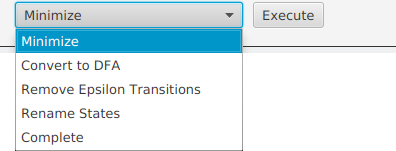
\includegraphics[width=0.75\textwidth]{bilder/gui4.png}
	\caption{Das Dropdown-Menü zeigt alle Plugins ohne grafische Oberfläche an}
	\label{fig:pic7}
\end{figure}
\newpage
\lstset{
	language=Java,
	breaklines=true,
	commentstyle=\color{green},
	keywordstyle=\color{blue},
	stringstyle=\color{magenta}
}
\section{Architektur und Erweiterung des Programms}\raggedbottom
\label{sec:3}
In diesem Abschnitt geht es um den Aufbau der Toolbox und wie man ihr neue Funktionen und Datentypen hinzufügen kann. Hiefür wird zunächst grob erläutert, wie die Ordnerstruktur des Programms aufgebaut ist und welche Klassen für welche Funktionen zuständig sind. Anschließend wird erläutert, wie Grammatiken und Automaten implementiert sind. Danach wird genauer auf die verschieden Interfaces eingegangen, mit denen neue Plugins erstellt werden können. Zuletzt wird noch erklärt, wie man dem Programm neue Datentypen hinzufügen kann.
\subsection{Aufbau der Toolbox}
\label{sec:3.1}
\paragraph{Wurzelverzeichnis}\ \\
Im Wurzelverzeichnis der Quellen liegen die beiden Java-Klassen \textit{GUI} und \textit{CLI}. Diese beiden Java-Klassen bilden das Hauptprogramm. \textit{GUI} ist dabei die Hauptklasse. Beim Start des Programms initialisiert sie die grafische Oberfläche und lädt alle Grafik-Plugins. Anschließend übergibt sie die Kontrolle an die Klasse \textit{CLI}. Diese lädt dann alle Konsolen-Plugins und startet die Kommandozeile. Nun kann der Benutzer Befehle eingeben. Die Befehle \textit{gui}, \textit{help} und \textit{exit} sind fest in CLI einprogrammiert, alle restlichen kommen von Plugins.
\paragraph{GrammarSimulator}\ \\
Dieses Verzeichnis enthält die Klassen, die eine Grammatik repräsentieren. Dazu gehören die Klasse \textit{Grammar}, welche eine Grammatik darstellt, das Interface \textit{Symbol} und die beiden Klassen \textit{Terminal} und \textit{Nonterminal}, welche \textit{Symbol} implementieren und Terminale, bzw. Nichtterminale repräsentieren.\\
Außerdem enthält dieser Ordner noch die Klasse \textit{GrammarUtil}, die viele Methoden beinhaltet, die mit Grammatiken arbeiten (zum Beispiel um die First- und Follow-Mengen einer Grammatik zu berechnen).
\paragraph{AutomatonSimulator}\ \\
In diesem Ordner befinden sich die Klassen, \textit{Automaton}, welche einen Automaten repräsentiert, \textit{State}, die einen Zustand darstellt und \textit{Rule}, die nötig ist um Produktionen zu speichern.\\
Des Weiteren befindet sich hier noch die Klasse \textit{AutomatonUtil}, die eine ähnliche Funktion wie \textit{GrammarUtil} hat, nur dass diese Algorithmen für Automaten und nicht für Grammatiken beinhaltet.
\paragraph{AutomatonParser und GrammarParser}\ \\
Diese beiden Ordner enthalten die von SableCC generierten Parser für Automaten und Grammatiken. Des Weiteren enthalten beide noch eine \textit{Visitor}-Klasse, welche aus einer geparsten Datei einen Automaten, bzw. eine Grammatik erstellt.
\paragraph{CLIPlugins}\ \\
Hier befindet sich das Interface \textit{CLIPlugin} und alle Konsolen-Plugins. Eine Klasse, die sich in diesem Verzeichnis befindet und das Interface CLIPlugin implementiert, wird von der Klasse \textit{CLI} automatisch zur Laufzeit geladen und kann vom Benutzer in der Konsole ausgeführt werden.
\paragraph{GUIPlugins}\ \\
Dieser Ordner beinhaltet nur die drei Unterverzeichnisse \textit{DisplayPlugins}, \textit{SimpleFunctionsPlugins} und \textit{ComplexFunctionPlugins}, die zusammen alle Plugins für die grafische Oberfläche enthalten.
\paragraph{GUIPlugins/DisplayPlugins}\ \\
Hier befindet das Interface \textit{DisplayPlugin}, sowie alle Klassen die es implementieren. Ein DisplayPlugin hat die Aufgabe einen bestimmten Datentypen grafisch darzustellen. Zu dem Plugin \textit{GrammarGUI}, welches Grammatiken darstellt, gibt es hier zusätzlich noch einen weiteren Unterordner \textit{GrammarTabs}.
\paragraph{DisplayPlugins/GUIPligins/GrammarTabs}\ \\
Wie in Abschnitt \hyperref[sec:2.4.1]{2.4.1} beschrieben, setzt sich die grafische Oberfläche für Grammatiken aus mehreren Tabs zusammen. Hierfür liegt in dem Unterordner \textit{GrammarTabs} das Interface \textit{GrammarTab} mit einigen Klassen, die es implementieren. Für jede dieser Klassen legt die Klasse \textit{GrammarGui} einen Tab in der Oberfläche an.
\paragraph{GUIPlugins/ComplexFunctionPlugins}\ \\
In diesem Verzeichnis liegt das Interface \textit{ComplexFunctionPlugin} zusammen mit den Klassen die es implementieren. Diese werden in der grafischen Oberfläche als die im Abschnitt \hyperref[sec:2.4.2.1]{2.4.2} beschrieben Plugins mit grafischer Oberfläche angezeigt.
\paragraph{GUIPlugins/SimpleFunctionPlugins}\ \\
Dieser Ordner enthält das Interface \textit{SimpleFunctionPlugin} und die Klassen die es implementieren. Diese Klassen werden in der grafischen Oberfläche in dem Dropdown-Menü unten rechts aufgelistet, so wie es im Abschnitt \hyperref[sec:2.4.2.2]{2.4.2} beschrieben wird.
\subsection{Implementierung von Grammatiken und Automaten}
\label{sec:3.2}
\paragraph{Grammatiken}\ \\
Eine Grammatik besteht in meiner Implementierung aus einem \lstinline[columns=fixed]{HashSet} von Nichtterminalen und einem \lstinline[columns=fixed]{HashSet} von Terminalen. Außerdem gibt es ein Nichttterminal, welches als Startsymbol ausgezeichnet ist.
\begin{lstlisting}[frame=single, basicstyle=\small, caption=Die Klasse \textit{Grammar}]
public class Grammar {
	private HashSet<Terminal> terminals;
	private HashSet<Nonterminal> nonterminals;
	private Nonterminal startSymbol;
	
	public Grammar() {
		Terminal terminal = new Terminal("a");
		ArrayList<Symbol> symbolList = new ArrayList(Arrays.asList(terminal));
		this.startSymbol = new Nonterminal("S", new HashSet<>(Arrays.asList(symbolList)));
		this.terminals = new HashSet<>(Arrays.asList(terminal));
		this.nonterminals = new HashSet<>(Arrays.asList(startSymbol));
	}
	
	public Grammar(HashSet<Terminal> terminals, HashSet<Nonterminal> nonterminals, Nonterminal startSymbol) {
		this.terminals = terminals;
		this.nonterminals = nonterminals;
		this.startSymbol = startSymbol;
	}
	
	public HashSet<Terminal> getTerminals() {
		return terminals;
	}
	
	public HashSet<Nonterminal> getNonterminals() {
		return nonterminals;
	}
	
	public Nonterminal getStartSymbol() {
		return startSymbol;
	}
	
	public void setStartSymbol(Nonterminal startSymbol) {
		this.startSymbol = startSymbol;
	}
}
\end{lstlisting}
Wie man sieht, gibt es zwei Konstruktoren. Einen, der keine Parameter nimmt und eine neue Grammatik erstellt, die nur das Nichtterminal \textit{S}, das Terminal \textit{a} und die Produktion \textit{S --> a} beinhaltet. Der zweite Konstruktor bekommt jeweils ein \lstinline[columns=fixed]{HashSet} von Terminalen und Nichtterminalen, sowie ein Nichtterminal, dass als Startsymbol fungieren soll.\\
Terminale und Nichtterminale werden jeweils durch eine eigenständige Klasse repräsentiert. Beide implementieren das Interface \lstinline[columns=fixed]{Symbol}:
\begin{lstlisting}[frame=single, basicstyle=\small, caption=Das Interface \textit{Symbol}]
public interface Symbol {
	String getName();
	void setName(String name);
}
\end{lstlisting}
Das Interface besteht nur aus einer Getter- und einer Setter-Methode für den Namen des \lstinline[columns=fixed]{Symbol}s, welcher in einem String gespeichert wird.\\
Die Klasse \lstinline[columns=fixed]{Terminal} implementiert \lstinline[columns=fixed]{Symbol} folgendermaßen:
\begin{lstlisting}[frame=single, basicstyle=\small, caption=Die Klasse \textit{Terminal}]
public class Terminal implements Symbol {
	private String name;
	
	public Terminal(String name) {
		this.name = name;
	}
	
	@Override
	public String getName() {
		return name;
	}
	
	@Override
	public void setName(String name) {
		this.name = name;
	}
}
\end{lstlisting}
Ein Terminal hat also nur einen Namen, der in der Variable \lstinline[columns=fixed]{name} gespeichert wird.\\
Ein Nichtterminal hingegen ist ein bisschen komplexer:
\begin{lstlisting}[frame=single, basicstyle=\small, caption=Die Klasse \textit{Nonterminal}]
public class Nonterminal implements Symbol {
	private String name;
	private HashSet<ArrayList<Symbol>> symbolLists;
	
	public Nonterminal(String name, HashSet<ArrayList<Symbol>> symbolLists) {
		this.name = name;
		this.symbolLists = symbolLists;
	}
	
	@Override
	public String getName() {
		return name;
	}
	
	@Override
	public void setName(String name) {
		this.name = name;
	}
	
	public HashSet<ArrayList<Symbol>> getSymbolLists() {
		return symbolLists;
	}
}
\end{lstlisting}
Zusätzlich zu dem Namen hat ein Nichtterminal noch ein \lstinline[columns=fixed]{HashSet} von \lstinline[columns=fixed]{ArrayLists} des Typs \lstinline[columns=fixed]{Symbol}. Diese Listen können somit sowohl Terminale, als auch Nichtterminale beinhalten und repräsentieren die rechte Seite einer Produktion, welche, wie in Abschnitt \hyperref[sec:1.1]{1.1} beschrieben, aus einer Folge von Terminalen und Nichtterminalen besteht.
\paragraph{Automaten}\ \\
Ein Automat hat ein \lstinline[columns=fixed]{HashSet} von Zuständen, ein \lstinline[columns=fixed]{HashSet} von Strings, wobei jeder String für ein mögliches Eingabesymbol steht, und einen als Startzustand markierten Zustand.
\begin{lstlisting}[frame=single, basicstyle=\small, caption=Die Klasse \textit{Automaton}]
public class Automaton {
	private HashSet<State> states;
	
	private State startState;
	private HashSet<String> allInputs;
	private boolean epsilonCycle = false;
	
	public Automaton(HashSet<State> states, State startState, HashSet<String> allInputs) {
		this.states = states;
		this.startState = startState;
		this.allInputs = allInputs;
		this.removeEpsilonCycles();
		if(epsilonCycle) {
			System.out.println("Epsilon-cycles in this automaton have been removed automatically!");
		}
	}
	
	public Automaton() {
		this.startState = new State("z0", true, false, new HashSet<>());
		this.states = new HashSet<>();
		this.states.add(this.startState);
		this.allInputs = new HashSet<>();
	}
	
	
	private void removeEpsilonCycles() {
		...
	}
	
	private void removeEpsilonCycles(State startState, HashSet<State> visitedStates, boolean cycleFound) {
		...
	}
	
	public HashSet<State> getStates() {
		return states;
	}
	
	public State getStartState() {
		return startState;
	}
	
	public HashSet<String> getAllInputs() {
		return allInputs;
	}
	
	public void setStartState(State startState) {
		this.startState = startState;
	}
}
\end{lstlisting}
Auch hier gibt es zwei Konstruktoren. Wie bei den Grammatiken gibt es einen, der keine Argumente nimmt. Dieser erstellt einen Automaten mit nur einem Zustand (dem Startzustand) und keinen Produktionen. Der andere bekommt eine Menge von Zuständen, eine Menge von möglichen Eingabesymbolen, und einen Startzustand. Mit Hilfe der Methode \lstinline[columns=fixed]{removeEpsilonCycles} werden alle zyklischen Epsilon-Produktionen entfernt (falls es welche gibt). Außerdem gibt es noch Getter-Methoden für die beiden \lstinline[columns=fixed]{HashSet}s und den Startzustand, sowie eine Setter-Methode für den Startzustand.\\
Zustände werden durch die Klasse \lstinline[columns=fixed]{State} repräsentiert:
\begin{lstlisting}[frame=single, basicstyle=\small, caption=Die Klasse \textit{State}]
public class State {
	private String name;	
	private boolean isStart;	
	private boolean isFinal;	
	private HashSet<Rule> rules;
	
	public State(String name, boolean isStart, boolean isFinal, HashSet<Rule> rules) {
		this.name = name;
		this.isStart = isStart;
		this.isFinal = isFinal;
		this.rules = rules;
	}
	
	public String getName() {
		return name;
	}
	
	public boolean isFinal() {
		return isFinal;
	}
	
	public boolean isStart() {
		return isStart;
	}
	
	public HashSet<Rule> getRules() {
		return rules;
	}
	
	public void setStart(boolean start) {
		isStart = start;
	}
	
	public void setFinal(boolean aFinal) {
		isFinal = aFinal;
	}
	
	public void setName(String name) {
		this.name = name;
	}
}
\end{lstlisting}
Ein Zustand besteht aus einem \lstinline[columns=fixed]{String}, der seinen Namen beinhaltet, zwei \lstinline[columns=fixed]{boolean}-Variablen, mit denen festgehalten wird, ob der Zustand ein Start-, bzw. Endzustand ist, und einem \lstinline[columns=fixed]{HashSet} vom Type \lstinline[columns=fixed]{Rule}, in welchem die Produktionen festgehalten sind, die von diesem Zustand ausgehen. Es gibt nur einen Konstruktor, der für jede der vier Variablen einen Wert übergeben bekommt. Zusätzlich gibt es noch einige Getter- und Setter-Methoden für die Variablen.\\
Produktionen werden durch die Klasse \lstinline[columns=fixed]{Rule} dargestellt:
\begin{lstlisting}[frame=single, basicstyle=\small, caption=Die Klasse \textit{Rule}]
public class Rule {
	private State goingTo;
	private HashSet<String> acceptedInputs;
	
	public Rule(State goingTo, HashSet<String> acceptedInputs) {
		this.goingTo = goingTo;
		this.acceptedInputs = acceptedInputs;
	}
	
	public State getGoingTo() {
		return goingTo;
	}
	
	public HashSet<String> getAcceptedInputs() {
		return acceptedInputs;
	}
	
	public void setGoingTo(State goingTo) {
		this.goingTo = goingTo;
	}
}
\end{lstlisting}
Eine Produktion besteht einfach nur aus dem Zustand auf den sie zeigt und einem \lstinline[columns=fixed]{HashSet} von Strings. Diese sind die Eingabesymbole, die von dieser Produktion akzeptiert werden.
\subsection{Erweiterung des Funktionsumfangs mit neuen Plugins}
\label{sec:3.3}
\subsubsection{Funktionen zur Kommandozeile hinzufügen mit \textit{CLIPlugin}}
\label{sec:3.3.1}
Um der Kommandozeile eine neue Funktion hinzuzufügen, muss eine neue Klasse im Ordner \textit{CLIPlugins} erstellt werden, die das Interface \lstinline[columns=fixed]{CLIPlugin} implementiert. \lstinline[columns=fixed]{CLIPlugin} besteht aus folgenden Methoden:
\begin{itemize}
	\item \lstinline[columns=fixed]{String[] getNames()}:\\
	Gibt ein Array aus Strings zurück. Wenn der Benutzer einen dieser Strings in die Kommandozeile eingibt, wird das Plugin ausgeführt.
	\item \lstinline[columns=fixed]{boolean checkParameters(String[] parameters)}:\\
	Als Parameter wird hier ein String-Array übergeben, das die Parameter, mit denen der Benutzer den Befehl aufgerufen hat, beinhaltet. Aufgabe dieser Methode ist es, diese auf ihre Gültigkeit zu prüfen und \lstinline[columns=fixed]{true} zurückzugeben, falls alles in Ordnung ist, bzw. \lstinline[columns=fixed]{false}, falls mit den Parametern etwas nicht stimmt.
	\item \lstinline[columns=fixed]{String getHelpText()}:\\
	Gibt den zu diesem Plugin zugehörigen Hilfetext zurück. Dieser wird ausgegeben, wenn der Benutzer den Befehl \textit{help} eintippt.
	\item \lstinline[columns=fixed]{Object execute(Object object, String parameters)}:\\
	Hier wird die eigentliche Funktion des Plugins implementiert. Als erster Parameter wird ein \lstinline[columns=fixed]{Object} übergeben. Dies kann zum Beispiel ein Automat sein und sollte vorher zu seinem eigentlichen Typen konvertiert werden. Der zweite Parameter ist ein \lstinline[columns=fixed]{String}-Array, welches die Parameter enthält, mit denen der Benutzer den Befehl aufgerufen hat. Der Rückgabewert ist auch vom Typ \lstinline[columns=fixed]{Object} und kann zum Beispiel wieder ein Automat sein, der durch das Plugin verändert wurde.
	\item \lstinline[columns=fixed]{Class inputType()}:\\
	Gibt ein Objekt vom Typ \lstinline[columns=fixed]{Class} zurück. Hierbei sollte es sich um den Klassentyp des Objekts handeln, dass die Methode \lstinline[columns=fixed]{execute(Object object, String parameters)} als ersten Parameter bekommen soll.
	\item \lstinline[columns=fixed]{Class outputType()}:\\
	Gibt ebenfalls ein Objekt vom Typ \lstinline[columns=fixed]{Class} zurück. Hierbei sollte es sich nun um den Klassentyp des Objekts handeln, dass \lstinline[columns=fixed]{execute(Object object, String parameters)} zurückgibt.
	\item \lstinline[columns=fixed]{boolean errorFlag()}:\\
	Diese Methode wird vom Hauptprogramm nach der Ausführung von \lstinline[columns=fixed]{execute(Object object, String[] parameters)} aufgerufen und gibt \lstinline[columns=fixed]{true} zurück, wenn die Ausführung erfolgreich war, bzw. \lstinline[columns=fixed]{false}, wenn dabei ein Fehler aufgetreten ist.
\end{itemize}
Zur Verdeutlichung wird nun nochmal anhand der Klasse \textit{AutomatonSavePlugin} gezeigt, wie ein Plugin für die Kommandozeile aussieht:
\lstset{
	language=Java,
	captionpos=b,
	breaklines=true,
	commentstyle=\color{green},
	keywordstyle=\color{blue},
	stringstyle=\color{magenta},
}
\begin{lstlisting}[frame=single, basicstyle=\small, caption=Der Kopf der Klasse \textit{AutomatonSavePlugin}]
public class AutomatonSavePlugin implements CLIPlugin {
	boolean errorFlag = false;
\end{lstlisting}
Wie man hier sieht, implementiert die Klasse \lstinline[columns=fixed]{AutomatonSavePlugin} das Interface \lstinline[columns=fixed]{CLIPlugin}. Als erstes wird dann in dieser Klasse die Variable \lstinline[columns=fixed]{errorFlag} vom Type \lstinline[columns=fixed]{boolean} mit dem Wert \lstinline[columns=fixed]{false} initialisiert. Diese wird später benötigt, um anzugeben, ob während der Ausführung des Plugins ein Fehler aufgetreten ist.
\begin{lstlisting}[frame=single, basicstyle=\small, caption=Die Methode \textit{getNames}]
@Override
public String[] getNames() {
	return new String[]{"sa", "save-automaton"};
}
\end{lstlisting}
Der Rückgabewert dieser Methode ist ein Array von \lstinline[columns=fixed]{String}s und enthält \lstinline[columns=fixed]{"sa"} und \lstinline[columns=fixed]{"save-automaton"}. Wenn der Benutzer einen dieser beiden \lstinline[columns=fixed]{String}s als Befehl in die Kommandozeile eingibt, wird das Plugin ausgeführt.
\begin{lstlisting}[frame=single, basicstyle=\small, caption=Die Methode \textit{checkParameters}]
@Override
public boolean checkParameters(String[] parameters) {
	if(parameters.length < 1) {
		System.out.println("Please enter a filename as parameter for this command!");
		return false;
	}
	return true;
}
\end{lstlisting}
Dieses Plugin erwartet einen Parameter, nämlich den Namen der Datei, bzw. den Pfad zu ihr, in die der aktuell geladene Automat gespeichert werden soll. Wird kein Parameter angegeben, schreibt die Methode eine Fehlermeldung in die Konsole und gibt \lstinline[columns=fixed]{false} zurück. Das Hauptprogramm weiß dann, dass der Benutzer eine fehlerhafte Eingabe gemacht hat und ruft nicht die Methode \lstinline[columns=fixed]{execute(Object object, String[] parameters)} auf. Ist alles in Ordnung, wird \lstinline[columns=fixed]{true} zurückgegeben.
\begin{lstlisting}[frame=single, basicstyle=\small, caption=Die Methode \textit{getHelpText}]
@Override
public String getHelpText() {
	return "Writes the loaded automaton into a text file, which can later be reloaded by this program. Takes a filename as parameter.";
}
\end{lstlisting}
Hier wird der Hilfetext dieses Plugins zurückgegeben.
\newpage
\begin{lstlisting}[frame=single, basicstyle=\small, caption=Die Methode \textit{execute}]
@Override
public Object execute(Object object, String[] parameters) {
	errorFlag = false;
	if(object == null) {
		System.out.println("Please use 'la', or 'load-automaton' to load an automaton before using this command!");
		errorFlag = true;
		return null;
	}
	Automaton automaton = (Automaton) object;
	AutomatonUtil.save(automaton, parameters[0]);
	return null;
}
\end{lstlisting}
Diese Methode ist das Herzstück des Plugins, da sie die eigentliche Funktion implementiert. Zunächst einmal wird überprüft, ob das übergebene Objekt gleich \lstinline[columns=fixed]{null} ist. Sollte dies der Fall sein, bedeutet das, dass noch kein Automat geladen wurde. Dementsprechend wird eine Fehlermeldung mit dem Hinweis ausgegeben, in dem der Benutzer gebeten wird einen Automaten zu laden, bevor er diesen Befehl benutzt. Anschließend wird die Variable \lstinline[columns=fixed]{errorFlag} auf \lstinline[columns=fixed]{true} gesetzt und \lstinline[columns=fixed]{null} zurückgegeben.\\
Wenn bereits ein Automat geladen wurde, wird \lstinline[columns=fixed]{object} mit einem Typecast zu einem Automaten umgewandelt und mit Hilfe der Methode \lstinline[columns=fixed]{save(Automaton automaton, String filename)} aus der Klasse \lstinline[columns=fixed]{AutomatonUtil} in eine Datei geschrieben. Da dieses Plugin keine Veränderungen an dem Automaten vornimmt, gibt es \lstinline[columns=fixed]{null} zurück.
\begin{lstlisting}[frame=single, basicstyle=\small, caption=Die Methode \textit{inputType}]
@Override
public Class inputType() {
	return Automaton.class;
}
\end{lstlisting}
Da dieses Plugin einen Automaten als ersten Parameter der Methode \lstinline[columns=fixed]{execute(Object object, String[] parameters)} haben möchte, wird hier \lstinline[columns=fixed]{Automaton.class} zurückgegeben.
\begin{lstlisting}[frame=single, basicstyle=\small, caption=Die Methode \textit{outputType}]
@Override
public Class outputType() {
	return null;
}
\end{lstlisting}
Wie oben bereis erwähnt, nimmt dieses Plugin keine Veränderungen an dem übergebenen Automaten vor. Deshalb wird hier einfach nur \lstinline[columns=fixed]{null} zurückgegeben. Dadurch weiß das Hauptprogramm, dass es den Rückgabewert von \lstinline[columns=fixed]{execute(Object object, String[] parameters)} verwerfen soll. Möchte man ein Plugin schreiben, das dauerhafte Veränderungen an einem Objekt vornimmt, so muss \lstinline[columns=fixed]{outputType()} den Typ dieses Objektes zurückgeben (in diesem Fall wäre dass \lstinline[columns=fixed]{Automaton.class}). Natürlich ist es auch möglich, dass ein Plugin zwei voneinander verschiedene Eingabe- und Ausgabetypen hat (zum Beispiel eine Grammatik als Eingabe, und eine Automaten als Ausgabe).
\begin{lstlisting}[frame=single, basicstyle=\small, caption=Die Methode \textit{errorFlag}]
@Override
public boolean errorFlag() {
	return errorFlag;
}
\end{lstlisting}
Diese Methode gibt einfach nur die Variable \lstinline[columns=fixed]{errorFlag} zurück.
\subsubsection{Erweiterung der grafischen Oberfläche mit \textit{DisplayPlugin}, \textit{SimpleFunctionPlugin} und \textit{ComplexFunctionPlugin}}
\label{sec:3.3.2}
Um der graphischen Oberfläche neue Funktionen hinzuzufügen gibt es drei Plugins.\\ \lstinline[columns=fixed]{DisplayPlugin} ist hierbei das Hauptinterface. Eine Klasse, die es implementiert, soll eine Datenstruktur (zum Beispiel einen Automaten) visuell darstellen und eventuell dem Benutzer die Möglichkeit geben diese zu bearbeiten.\\
Mit \lstinline[columns=fixed]{SimpleFunctionPlugin} und \lstinline[columns=fixed]{ComplexFunctionPlugin} können Funktionen hinzugefügt werden, die mit einer bestimmten Datenstruktur arbeiten (zum Beispiel ein Plugin, das einen Automaten minimiert).
\paragraph{Das Interface DisplayPlugin}\ \\
Um der Toolbox um ein neues \lstinline[columns=fixed]{DisplayPlugin} zu erweitern, muss eine Klasse im Ordner \textit{GUIPlugins/DisplayPlugins} erstellt werden, die \lstinline[columns=fixed]{DisplayPlugin} implementiert. Hierzu müssen folgende Methoden implementiert werden:
\begin{itemize}
	\item \lstinline[columns=fixed]{Node display(Object object)}:\\
	Diese Methode soll das ihr übergebene Objekt auf einem JavaFX-\lstinline[columns=fixed]{Node} visualisieren. Üblicherweise nimmt man hierzu ein \lstinline[columns=fixed]{Pane}, es kann aber irgendein Objekt zurückgegeben werden, das von \lstinline[columns=fixed]{Node} erbt. Somit ist es auch möglich das übergebene Objekt mit Hilfe von Swing darzustellen. Man muss dafür nur das Haupt-\lstinline[columns=fixed]{JPanel} auf ein \lstinline[columns=fixed]{SwingNode} legen.
	\item \lstinline[columns=fixed]{void refresh(Object object)}:\\
	Die \lstinline[columns=fixed]{refresh}-Methode wird vom Hauptprogramm aufgerufen, wenn das Objekt, das von diesem Plugin dargestellt wird, verändert wurde. Die Methode soll dann die Darstellung des Objekts aktualisieren.
	\item \lstinline[columns=fixed]{Object newObject()}:\\
	Diese Methode soll ein neues Objekt erstellen und zurückgeben.
	\item \lstinline[columns=fixed]{Object openFile()}:\\
	Der Benutzer wird gebeten eine Datei zu öffnen (zum Beispiel mit einem \lstinline[columns=fixed]{FileChooser}). Diese Datei soll dann geparst und das resultierende Objekt zurückgegeben werden.
	\item \lstinline[columns=fixed]{void saveFile(Object object)}:\\
	Speichert das übergebene Objekt in einer Datei. Vorher soll der User noch nach dem Pfad und Namen der Datei gefragt werden (zum Beispiel mit einem \lstinline[columns=fixed]{FileChooser}).
	\item \lstinline[columns=fixed]{String getName()}:\\
	Gibt den Namen dieses Plugins als String zurück. Dieser wird im \textit{ChoosePlugin}-Menü angezeigt.
	\item \lstinline[columns=fixed]{Class displayType()}:\\
	Diese Methode gibt den Klassentypen der Objekte zurück, die dieses Plugin darstellen kann.
\end{itemize}
Um detailliert zu zeigen, wie ein solches Plugin implementiert wird, folgt nun ein einfaches Beispiel-Plugin, welches alle Produktion einer Grammatik anzeigt:
\begin{lstlisting}[frame=single, basicstyle=\small, caption=Der Kopf der Klasse \textit{GrammarExample}]
public class GrammarExample implements DisplayPlugin {
	GridPane rootPane;
\end{lstlisting}
Auf dem \lstinline[columns=fixed]{GridPane rootPane} sollen die Produktion dargestellt werden.
\begin{lstlisting}[frame=single, basicstyle=\small, caption=Die Methode \textit{displayRules}]
private void displayRules(Grammar grammar) {
	rootPane.getChildren().clear();
	
	int i = 0;
	for(Nonterminal nonterminal : GrammarUtil.getNonterminalsInOrder(grammar)) {
		for(ArrayList<Symbol> symbolList : nonterminal.getSymbolLists()) {
			StringBuilder sb = new StringBuilder();
			Iterator<Symbol> it = symbolList.iterator();
			while(it.hasNext()) {
			sb.append(it.next().getName());
			if(it.hasNext()) {
				sb.append(", ");
			}
		}
		
		rootPane.add(new Label(nonterminal.getName()), 0, i);
		rootPane.add(new Label("-->"), 1, i);
		rootPane.add(new Label(sb.toString()), 2, i);
		i++;
		}
	}
}
\end{lstlisting}
\lstinline[columns=fixed]{displayRules(Grammar grammar)} ist eine Hilfsmethode, die als Parameter eine Grammatik bekommt und deren Produktionen in Form von \lstinline[columns=fixed]{Label}s auf dem \lstinline[columns=fixed]{rootPane} darstellt. Dabei wird die Methode \lstinline[columns=fixed]{getNonterminalsInOrder(Grammar grammar)} aus der Klasse \lstinline[columns=fixed]{GrammarUtil} verwendet, damit die Produktionen nach den Nichtterminalen, die auf der linken Seite stehen, sortiert sind. Prinzipiell könnte man auch einfach über \lstinline[columns=fixed]{grammar.getNonterminals()} iterieren, jedoch wäre die Reihenfolge der Produktionen dann zufällig.\\
Der Rest der Methode sollte relativ einfach verständlich sein. Für jede Symbolliste auf die ein Nichtterminal zeigt, werden drei Labels angelegt, die den Namen des Nichtterminals, einen Pfeil und die Symbolliste enthalten. Anschließend werden dieses Labels in eine neue Zeile auf dem \lstinline[columns=fixed]{rootPane} gelegt.
\begin{lstlisting}[frame=single, basicstyle=\small, caption=Die Methode \textit{display}]
@Override
public Node display(Object object) {
	Grammar grammar = (Grammar) object;
	rootPane = new GridPane();
	rootPane.setAlignment(Pos.CENTER);
	rootPane.setHgap(10);
	rootPane.setVgap(5);
	displayRules(grammar);
	return rootPane;
}
\end{lstlisting}
Die \lstinline[columns=fixed]{display(Object object)}-Methode wandelt zunächst das ihr übergebene Objekt in eine Grammatik um und initialisiert dann das \lstinline[columns=fixed]{rootPane}. Anschließend werden noch einige Attribute des \lstinline[columns=fixed]{rootPane}s verändert, damit die auf ihm liegenden Objekte zentriert sind und einige Pixel Abstand zueinander haben. Zuletzt wird das \lstinline[columns=fixed]{rootPane} mit Hilfe von \lstinline[columns=fixed]{displayRules(Grammar grammar)} gefüllt und danach zurückgegeben.
\begin{lstlisting}[frame=single, basicstyle=\small, caption=Die Methode \textit{refresh}]
@Override
public void refresh(Object object) {
	displayRules((Grammar) object);
}
\end{lstlisting}
Um die Oberfläche zu aktualisieren, muss \lstinline[columns=fixed]{displayRules(Grammar grammar)} aufgerufen werden.
\begin{lstlisting}[frame=single, basicstyle=\small, caption=Die Methode \textit{newObject}]
@Override
public Object newObject() {
	return new Grammar();
}
\end{lstlisting}
Um eine neue Grammatik zu erzeugen, reicht es den Konstruktor der Klasse \lstinline[columns=fixed]{Grammar} ohne Argumente aufzurufen. Dieser erstellt dann automatisch eine neue Grammatik mit einem Terminal, einem Nichtterminal und einer Produktion.
\begin{lstlisting}[frame=single, basicstyle=\small, caption=Die Methode \textit{openFile}]
@Override
public Object openFile() {
	FileChooser chooser = new FileChooser();
	chooser.setTitle("Open file");
	File selectedFile = chooser.showOpenDialog(new Stage());
	String fileInput = "";
	try {
		BufferedReader reader = new BufferedReader(new FileReader(selectedFile.getName()));
		String line;
		while ((line = reader.readLine()) != null) {
			fileInput = fileInput + line + "\n";
		}
		return GrammarUtil.parse(fileInput);
	} catch (Exception e) {
		Alert alert = new Alert(Alert.AlertType.ERROR);
		alert.setTitle("STUPS-Toolbox");
		alert.setHeaderText("Error while opening the file!");
		alert.showAndWait();
		return null;
	}
}
\end{lstlisting}
In \lstinline[columns=fixed]{openFile()} wird zu Beginn ein FileChooser initialisiert. Im \lstinline[columns=fixed]{try}-Block wird dieser dann angezeigt und der Inhalt der ausgewählten Datei wird in die Variable \lstinline[columns=fixed]{fileInput eingelesen}. Anschließend wird dieser mit der Methode \lstinline[columns=fixed]{parse(String fileInput)} aus der Klasse \lstinline[columns=fixed]{GrammarUtil} zu einer Grammatik geparst. Die Grammatik muss dafür in dem in Abschnitt \hyperref[sec:2.1]{2.1} beschriebenen Format vorliegen. Sollte dabei etwas schief gehen, wird im \lstinline[columns=fixed]{catch}-Block ein Fenster mit einer einfachen Fehlermeldung angezeigt.
\begin{lstlisting}[frame=single, basicstyle=\small, caption=Die Methode \textit{saveFile}]
@Override
public void saveFile(Object object) {
	FileChooser chooser = new FileChooser();
	chooser.setTitle("Save file");
	File selectedFile = chooser.showSaveDialog(new Stage());
	if(selectedFile != null) {
		GrammarUtil.save((Grammar) object, selectedFile.getAbsolutePath());
	}
}
\end{lstlisting}
Genau wie in \lstinline[columns=fixed]{openFile()} wird hier zunächst ein FileChooser angezeigt. Der Pfad zu der ausgewählten Datei wird dann der Methode \lstinline[columns=fixed]{save(Grammar grammar, String path)} aus der Klasse \lstinline[columns=fixed]{GrammarUtil} übergeben, welche die aktuelle Grammatik in diese Datei schreibt. Dabei wird das in Abschnitt \hyperref[sec:2.1]{2.1} beschriebene Format verwendet.
\begin{lstlisting}[frame=single, basicstyle=\small, caption=Die Methode \textit{menus}]
@Override
public HashSet<Menu> menus(Object object, Node node) {
	MenuItem helpItem = new MenuItem("Help");
	MenuItem aboutItem = new MenuItem("About Plugin");
	
	helpItem.setOnAction(event -> {
		Alert alert = new Alert(Alert.AlertType.INFORMATION);
		alert.setTitle("STUPS-Toolbox");
		alert.setHeaderText("This is just a simple example plugin,\nthat displays all productions of the loaded grammar.");
		alert.showAndWait();
	});
	
	aboutItem.setOnAction(event -> {
		Alert alert = new Alert(Alert.AlertType.INFORMATION);
		alert.setTitle("STUPS-Toolbox");
		alert.setHeaderText("Grammar Example Plugin v1.0");
		alert.showAndWait();
	});
	
	Menu aboutMenu = new Menu("Help");
	aboutMenu.getItems().addAll(helpItem, aboutItem);
	
	return new HashSet<>(Arrays.asList(aboutMenu));
}
\end{lstlisting}
Hier werden zwei \lstinline[columns=fixed]{MenuItem}s erstellt, die einen kurzen Hilfetext, bzw. eine Versionsnummer anzeigen, wenn der Benutzer auf sie klickt. Anschließend werden diese einem \lstinline[columns=fixed]{Menu}-Objekt hinzugefügt und dieses als Teil eines \lstinline[columns=fixed]{HashSet}s zurückgegeben. Das Hauptprogramm fügt alle Objekte in diesem \lstinline[columns=fixed]{HashSet} in die Menüleiste ein, wenn das Plugin ausgewählt wird.
\begin{lstlisting}[frame=single, basicstyle=\small, caption=Die Methode \textit{getName}]
@Override
public String getName() {
	return "Grammar Example";
}
\end{lstlisting}
\lstinline[columns=fixed]{getName()} gibt den Namen des Plugins als String zurück.
\begin{lstlisting}[frame=single, basicstyle=\small, caption=Die Methode \textit{displayType}]
@Override
public Class displayType() {
	return Grammar.class;
}
\end{lstlisting}
Dieses Plugin arbeitet mit Grammatiken, dementsprechend wird hier \lstinline[columns=fixed]{Grammar.class} zurückgegeben.
\paragraph{Das Grammatik-Plugin erweitern mit dem Interface \textit{GrammarTab}}\ \\
Da es noch viele weitere Funktionen gibt, die der Grammatikoberfläche hinzugefügt werden könnten, habe ich mich dazu entschlossen das Plugin \lstinline[columns=fixed]{GrammarGUI} ebenfalls erweiterbar zu gestalten. Hierfür gibt es ein sehr einfaches Interface, welches ein Objekt vom Typ \lstinline[columns=fixed]{Node} erstellt. Dieses wird dann dem \lstinline[columns=fixed]{TabbedPane} von \lstinline[columns=fixed]{GrammarGUI} hinzugefügt. Das Interface \lstinline[columns=fixed]{GrammarTab} liegt im Ordner \textit{GUIPlugins/DisplayPlugins/GrammarTabs} und alle Klassen, die es implementieren, müssen sich ebenfalls in diesem Ordner befinden. Es besteht nur aus den folgenden zwei Methoden:
\begin{itemize}
	\item \lstinline[columns=fixed]{Node getFxNode(Grammar grammar)}:\\
	Diese Methode macht das Gleiche, wie die oben beschriebene Methode \lstinline[columns=fixed]{display(Object object)} aus dem Interface \lstinline[columns=fixed]{DisplayPlugin}, indem sie ein Objekt vom Type \lstinline[columns=fixed]{Node} zurückgibt. Dieses wird in der Oberfläche für Grammatiken in einem eigenen Tab angezeigt.
	\item \lstinline[columns=fixed]{String getName()}:\\
	\lstinline[columns=fixed]{getName()} gibt den Namen des Tabs zurück. Dieser wird in der Oberfläche angezeigt.
\end{itemize}
\paragraph{Das Interface \textit{SimpleFunctionPlugin}}\ \\
Mit dem Interface \lstinline[columns=fixed]{SimpleFunctionPlugin} ist es möglich der grafischen Oberfläche neue Funktionen hinzuzufügen, die ein Objekt (zum Beispiel eine Grammatik) als Eingabe nehmen, und dieses verändern. Das neue Objekt wird dann direkt in der Oberfläche angezeigt. Diese Plugins werden unten rechts in einem Dropdown-Menü angezeigt (wie in Abschnitt \hyperref[sec:2.4.2]{2.4.2} beschrieben). \lstinline[columns=fixed]{SimpleFunctionPlugin} besteht aus den folgenden vier Methoden:
\begin{itemize}
	\item \lstinline[columns=fixed]{Object execute(Object object)}:\\
	Als Parameter wird hier ein Objekt von dem Typ übergeben, mit dem dieses Plugin arbeitet. Der Rückgabewert dieser Methode ist das veränderte Objekt, oder sogar ein Objekt von einem ganz anderem Typ. Dies funktioniert genauso wie beim Interface \lstinline[columns=fixed]{CLIPlugin}.
	\item \lstinline[columns=fixed]{String getName()}:\\
	Der Rückgabewert dieser Methode ist ein String mit dem Namen des Plugins. Dieser wird in dem Dropdown-Menü angezeigt.
	\item \lstinline[columns=fixed]{Class inputType()}:\\
	Diese Methode gibt den Klassentyp des Eingabeobjekts von \lstinline[columns=fixed]{Object execute(Object object)} zurück. Das Plugin wird nur angezeigt, wenn der Rückgabewert von \lstinline[columns=fixed]{inputType()} mit dem Rückgabewert der Methode \lstinline[columns=fixed]{displayType()} des aktuell angezeigten \lstinline[columns=fixed]{DisplayPlugin}s übereinstimmt.
	\item \lstinline[columns=fixed]{Class outputType()}:\\
	Diese Methode gibt den Klassentyp des Rückgabewertes von \lstinline[columns=fixed]{Object execute(Object object)} zurück. Dieser muss nicht gleich dem Eingabetypen sein.
\end{itemize}
\newpage
Diese Methoden werden nun anhand der Klasse \lstinline[columns=fixed]{AutomatonConvertToDFAPlugin} weiter erläutert:
\begin{lstlisting}[frame=single, basicstyle=\small, caption=Die Methode \textit{execute}]
@Override
public Object execute(Object object) {
	Automaton automaton = (Automaton) object;
	return AutomatonUtil.convertToDFA(automaton);
}
\end{lstlisting}
Das übergebene Objekt wird zunächst per Typecast in einen Automaten umgewandelt. Anschließend wird dieser Automat mit Hilfe der Methode \lstinline[columns=fixed]{convertToDFA(Automaton automaton)} aus der Klasse \lstinline[columns=fixed]{AutomatonUtil} in einen DFA umgewandelt und zurückgegeben.
\begin{lstlisting}[frame=single, basicstyle=\small, caption=Die Methode \textit{getName}]
@Override
public String getName() {
	return "Convert to DFA";
}
\end{lstlisting}
Die Methode gibt einfach nur den Namen des Plugins als String zurück. In dem Dropdown-Menü erscheint nun der Eintrag \textit{Convert to DFA}.
\begin{lstlisting}[frame=single, basicstyle=\small, caption=Die Methode \textit{inputType}]
@Override
public Class inputType() {
	return Automaton.class;
}
\end{lstlisting}
\lstinline[columns=fixed]{Object execute(Object object)} erwartet einen Automaten als Parameter, dementsprechend wird hier \lstinline[columns=fixed]{Automaton.class} zurückgegeben.
\begin{lstlisting}[frame=single, basicstyle=\small, caption=Die Methode \textit{outputType}]
@Override
public Class outputType() {
	return Automaton.class;
}
\end{lstlisting}
Der Rückgabetyp von \lstinline[columns=fixed]{Object execute(Object object)} ist ebenfalls ein Automat, deshalb wird hier auch \lstinline[columns=fixed]{Automaton.class} zurückgegeben.
\paragraph{Das Interface \textit{ComplexFunctionPlugin}}\ \\
Mit dem Interface \lstinline[columns=fixed]{ComplexFunctionPlugin} ist es möglich der grafischen Oberfläche neue Funktionen hinzuzufügen, die ihrerseits eine eigene Oberfläche besitzen. Diese werden, wie in Abschnitt \hyperref[sec:2.4.2]{2.4.2} beschrieben, unten links in der grafischen Oberfläche angezeigt. Des Weiteren bekommen diese Plugins eine Instanz des gerade angezeigten \lstinline[columns=fixed]{DisplayPlugin}s, so dass es mit diesem zusammenarbeiten kann. Dadurch ist es natürlich auch an ein bestimmtes \lstinline[columns=fixed]{DisplayPlugin} gebunden. \lstinline[columns=fixed]{ComplexFunctionPlugin} setzt sich aus den folgenden drei Methoden zusammen:
\begin{itemize}
	\item \lstinline[columns=fixed]{Node getFxNode(Object object, DisplayPlugin GUI)}:\\
	Ähnlich wie bei dem Interface \lstinline[columns=fixed]{GrammarTab} wird hier ein Objekt vom Type \lstinline[columns=fixed]{Node} zurückgegeben, das in der grafischen Oberfläche angezeigt werden soll. Als Parameter werden ein Objekt (zum Beispiel eine Grammatik, oder ein Automat) und ein DisplayPlugin übergeben. So kann diese Methode auf Ressourcen des DisplayPlugins zugreifen. Wie das genau funktionieren kann, wird weiter unten anhand eines Beispiels gezeigt.
	\item \lstinline[columns=fixed]{String getName()}:\\
	Gibt den Namen des Plugins als String zurück. Dieser wird oberhalb des in \lstinline[columns=fixed]{getFxNode(Object object, DisplayPlugin GUI)} zurückgegeben \lstinline[columns=fixed]{Node}s in einem \lstinline[columns=fixed]{Label} angezeigt.
	\item \lstinline[columns=fixed]{Class displayPluginType()}:\\
	Hier wird der Klassentyp des \lstinline[columns=fixed]{DisplayPlugin}s, welches \lstinline[columns=fixed]{getFxNode(Object object, DisplayPlugin GUI)} als zweiter Parameter übergeben wird zurückgegeben. Dieses Plugin wird nur angezeigt, wenn das aktuell angezeigte \lstinline[columns=fixed]{DisplayPlugin} den hier zurückgegeben Typen hat.
\end{itemize}
Wie die Zusammenarbeit zwischen einem \lstinline[columns=fixed]{ComplexFunctionPlugin} und einem \lstinline[columns=fixed]{DisplayPlugin} laufen könnte, wird nun durch ein kurzes Beispiel-Plugin gezeigt, mit welchem der Benutzer ein anderes Layout für den Übergangsgraphen wählen kann:
\begin{lstlisting}[frame=single, basicstyle=\small, caption=Die Methode \textit{getFxNode}]
@Override
public Node getFxNode(Object object, DisplayPlugin GUI) {
	AutomatonGUI automatonGUI = (AutomatonGUI) GUI;
	VisualizationViewer<String, Integer> viewer = automatonGUI.getVisualizationViewer();
	Graph<String, Integer> graph = automatonGUI.getGraph();
	
	MenuBar menuBar = new MenuBar();
	Menu layoutMenu = new Menu("Choose Layout");
	
	MenuItem circleLayout = new MenuItem("Circle Layout");
	MenuItem frLayout = new MenuItem("FR Layout 1");
	MenuItem frLayout2 = new MenuItem("FR Layout 2");
	MenuItem isomLayout = new MenuItem("ISOM Layout");
	MenuItem kkLayout = new MenuItem("KK Layout");
	
	circleLayout.setOnAction(event -> viewer.setGraphLayout(new CircleLayout<>(graph)));
	frLayout.setOnAction(event -> viewer.setGraphLayout(new FRLayout<>(graph)));
	frLayout2.setOnAction(event -> viewer.setGraphLayout(new FRLayout2<>(graph)));
	isomLayout.setOnAction(event -> viewer.setGraphLayout(new ISOMLayout<>(graph)));
	kkLayout.setOnAction(event -> viewer.setGraphLayout(new KKLayout<>(graph)));
	
	layoutMenu.getItems().addAll(circleLayout, frLayout, frLayout2, isomLayout, kkLayout);
	menuBar.getMenus().add(layoutMenu);
	
	return menuBar;
}
\end{lstlisting}
Im ersten Schritt wird das übergebene \lstinline[columns=fixed]{DisplayPlugin} in eine Instanz von \lstinline[columns=fixed]{AutomatonGUI} umgewandelt und die benötigten Ressourcen daraus geholt. Diese sind der \lstinline[columns=fixed]{VisualizationViewer} und der \lstinline[columns=fixed]{Graph}. Anschließend wird ein Menü mit fünf Einträgen für die verschiedenen Layouts initialisiert. Die \lstinline[columns=fixed]{setOnAction(EventHandler<ActionEvent> value)}-Methode jedes Menüeintrags ändert das Layout des \lstinline[columns=fixed]{VisualizationViewer}s zu einem bestimmten Layout. Zuletzt werden die Menüeinträge dem Menü hinzugefügt, das Menü in eine \lstinline[columns=fixed]{MenuBar} gepackt und diese zuürckgegeben.
\begin{lstlisting}[frame=single, basicstyle=\small, caption=Die Methode \textit{getName}]
@Override
public String getName() {
	return "Layout Example";
}
\end{lstlisting}
Hier wird der Anzeigename des Plugins festgelegt.
\begin{lstlisting}[frame=single, basicstyle=\small, caption=Die Methode \textit{displayPluginType}]
@Override
public Class displayPluginType() {
	return AutomatonGUI.class;
}
\end{lstlisting}
Dieses Plugin soll nur angezeigt werden, wenn das \lstinline[columns=fixed]{DisplayPLugin} \lstinline[columns=fixed]{AutomatonGUI} angezeigt wird. Dementsprechend wird hier \lstinline[columns=fixed]{AutomatonGUI.class} zurückgegeben.
\paragraph{Optionalität der Plugins}\ \\
Die Benutzung der Interfaces \lstinline[columns=fixed]{SimpleFunctionPlugin} und \lstinline[columns=fixed]{ComplexFunctionPlugin} ist bei der Entwicklung neuer grafischer Oberflächen optional. Es ist auch möglich, alle Funktionen direkt in das \lstinline[columns=fixed]{DisplayPlugin} einzubauen. Jedoch bieten die beiden Interfaces eine einfache Möglichkeit neue Oberflächen übersichtlich und modular zu programmieren.
\subsection{Die Toolbox um neue Datentypen erweitern}
\label{sec:3.4}
Neue Datentypen zum Programm hinzuzufügen ist sehr einfach. Die Klasse \lstinline[columns=fixed]{CLI} hat ein \lstinline[columns=fixed]{HashSet} von Objekten. Wenn ein Plugin ein Objekt von einem Datentyp zurückgibt, der noch nicht in diesem \lstinline[columns=fixed]{HashSet} vorkommt, wird es ihm hinzugefügt. Falls es bereits ein Objekt diesen Datentyps gibt, wird dieser Eintrag im \lstinline[columns=fixed]{HashSet} durch das neue Objekt ersetzt. Das Ganze funktioniert völlig unabhängig davon, welchen Datentyp ein Objekt hat.\\
Um nun einen neuen Datentyp hinzuzufügen, muss man nur irgendwo im Programm eine Klasse erstellen, die den neuen Datentypen repräsentiert. Sobald es ein Plugin gibt, das ein Objekt von diesesm Datentyp zurückgibt, ist dieser im Programm.
\newpage
\section{Fazit}\raggedbottom
Ziel dieser Bachelorarbeit war es, ein Programm zu erstellen, welches Studenten, die gerade erst mit dem Studium der Theoretischen Informatik begonnen haben, beim Lernen unterstützt. Das tut die im Rahmen dieser Arbeit programmierte Toolbox auch, man muss jedoch darauf achten, wie man sie benutzt. Die Möglichkeit Automaten zu visualisieren und zu bearbeiten ist sicherlich hilfreich, wenn man gerade erst angefangen hat, etwas über sie zu lernen. Zudem ist es auch möglich, einen Automaten Zustand für Zustand und Produktion für Produktion aufzubauen und die \textit{Check String}-Funktion ermöglicht es Schritt für Schritt zu simulieren, wie ein Automat einen Eingabestring verarbeitet. Wenn man jedoch das Programm einfach nur benutzt um Aufgaben zu lösen ohne darüber nachzudenken, ist dies wenig hilfreich für den Lernerfolg.\\
Bei der Simulation von Grammatiken fehlen sicherlich noch einige Funktionen, wie zum Beispiel das Umwandeln einer Grammatik in die Chomsky-Normalform und der CYK-Algorithmus. Da jedoch von vornherein abzusehen war, dass in drei Monaten Entwicklungszeit nur eine begrenzte Anzahl von Funktionen implementiert werden kann, wurde als weiteres Ziel gesetzt, dass die Toolbox einfach erweiterbar sein soll. Dies ist durch das von mir entwickelte Plugin-System gewährleistet. Der modulare Aufbau der grafischen Oberfläche macht die Entwicklung von neuen Plugins flexibel und einfach, ohne zukünftige Entwickler einzuschränken.

%%%%%%%%%%%%%%%%%%%%%%%%%%%%%%%%%%%%%%%%%%%%%%%%%%%%%%%%%%%%%%%%%%%%%%%%
%%%% ENDE TEXTTEIL %%%%%%%%%%%%%%%%%%%%%%%%%%%%%%%%%%%%%%%%%%%%%%%%%%%%%
%%%%%%%%%%%%%%%%%%%%%%%%%%%%%%%%%%%%%%%%%%%%%%%%%%%%%%%%%%%%%%%%%%%%%%%%

\clearpage

% Entfernen Sie das Kommentar aus der nachfolgenden Zeile, falls Sie einen Anhang in der Arbeit verwenden wollen. Beachten Sie, dass Sie sich im Verlauf der Arbeit mit \ref{...} (z.B. \ref{anhang:zusatz1}) auf den Anhang beziehen.
\newpage
\appendix
\section{Anhang}
\subsection*{JUNG2-Lizenz} \label{anhang:zusatz1}
Zum Anzeigen von Automaten wird die Java-Bibliothek \textit{JUNG2} verwendet. Diese steht unter der \textit{BSD open-source} Lizenz:
\lstset{
	captionpos=b,
	breaklines=true,
	basicstyle=\footnotesize,
	language={}
}
\begin{lstlisting}[frame=single, caption=Die \textit{BSD open-source} Lizenz]
The license below is the BSD open-source license. See 
http://www.opensource.org/licenses/bsd-license.php
with:
<OWNER> = Regents of the University of California and the JUNG Project
<ORGANIZATION> = University of California
<YEAR> = 2003 

It allows redistribution of JUNG freely, albeit with acknowledgement of JUNG's being a component in the redistributed software. However, we would greatly appreciate if you can let us know what you are doing with JUNG.

--
THE JUNG LICENSE

Copyright (c) 2003-2004,  Regents of the University of California and the JUNG Project 
All rights reserved.

Redistribution and use in source and binary forms, with or without modification, are permitted provided that the following conditions are met:

* Redistributions of source code must retain the above copyright notice, this list of conditions and the following disclaimer.
* Redistributions in binary form must reproduce the above copyright notice, this list of conditions and the following disclaimer in the documentation and/or other materials provided with the distribution.
* Neither the name of the University of California nor the names of its contributors may be used to endorse or promote products derived from this software without specific prior written permission.

THIS SOFTWARE IS PROVIDED BY THE COPYRIGHT HOLDERS AND CONTRIBUTORS "AS IS" AND ANY EXPRESS OR IMPLIED WARRANTIES, INCLUDING, BUT NOT LIMITED TO, THE IMPLIED WARRANTIES OF MERCHANTABILITY AND FITNESS FOR A PARTICULAR PURPOSE ARE DISCLAIMED. IN NO EVENT SHALL THE COPYRIGHT OWNER OR CONTRIBUTORS BE LIABLE FOR ANY DIRECT, INDIRECT, INCIDENTAL, SPECIAL, EXEMPLARY, OR CONSEQUENTIAL DAMAGES (INCLUDING, BUT NOT LIMITED TO, PROCUREMENT OF SUBSTITUTE GOODS OR SERVICES; LOSS OF USE, DATA, OR PROFITS; OR BUSINESS INTERRUPTION) HOWEVER CAUSED AND ON ANY THEORY OF LIABILITY, WHETHER IN CONTRACT, STRICT LIABILITY, OR TORT (INCLUDING NEGLIGENCE OR OTHERWISE) ARISING IN ANY WAY OUT OF THE USE OF THIS SOFTWARE, EVEN IF ADVISED OF THE POSSIBILITY OF SUCH DAMAGE.
\end{lstlisting}
\clearpage

\bibliography{references}
\bibliographystyle{alphadin}
%\vspace*{\fill}

\clearpage

\listoffigures

\listoftables

\lstlistoflistings
%\pagebreak

%\printindex
\end{document}
